\subsection{Homework 4}
\begin{enumerate}
    \item The data in the following table consists of scores of 20 children with neurological disorders. The two tests, A and B, are both tests of spatial perception ([Efron and Tibshirani, 1993]). The scales of the two tests are the same: they both have a range of 0 to 50. Psychologists often use two versions of a test that they hope measure the same thing, because this gives them the opportunity to test people multiple times. Psychologists often want to compare scores over time, but if researchers give the same test twice, any improvements may be due simply to memory of the previous test. If we have two tests, one thing we might want to know is whether the means of the scores are different.
    \FloatBarrier
    \begin{table}[h]
    \centering
    \begin{tabular}{@{}ccc||ccc@{}}
    Person & Test A & Test B & Person & Test A & Test B \\ \hline
    1 & 48 & 42 & 11 & 45 & 34 \\
    2 & 36 & 33 & 12 & 14 & 22 \\
    3 & 20 & 16 & 13 & 6 & 7 \\
    4 & 29 & 39 & 14 & 0 & 15 \\
    5 & 42 & 38 & 15 & 33 & 34 \\
    6 & 42 & 36 & 16 & 28 & 29 \\
    7 & 20 & 15 & 17 & 34 & 41 \\
    8 & 42 & 33 & 18 & 4 & 13 \\
    9 & 22 & 20 & 19 & 32 & 38 \\
    10 & 41 & 43 & 20 & 24 & 25
    \end{tabular}
    \caption{}
    \label{tab:hw4q1}
    \end{table}
    \FloatBarrier
    By computing the differences between Test A and Test B for each person, we can see that the mean difference between Test A and B (Test A minus Test B) equals $-0.55$, and that the standard deviation of the difference is 6.886.
    \begin{enumerate}
        \item Suppose that we would like to show that the scores on Test A and B in the population are, on average, the same. A naive researcher would like to use a significance test for this. Give the hypotheses that the researcher will use, $H_0$ and $H_A$; describe the meaning of the parameters you use in your hypotheses.
        \begin{framed}{\textbf{Solution}}
        The information that we are given is that $\bar{d} = -0.55$ and $s_d = 6.886$, where $D = A - B$ is the random variable denoting the difference between the random variables $A$ and $B$ which are the scores on test $A$ and $B$, respectively. Also, $n=20$ and each test has a maximum score of 50. The naive researcher might be testing:
        \[
            \begin{matrix}
            H_0 & : & \mu_d = 0 \\
            H_A & : & \mu_d \ne 0.
            \end{matrix}
        \]
        It is crucial to understand why we have selected a two-tailed significance test here! Both tests are supposedly equal in their outcomes, so we do not assume that either test provides a different answer. Moreover they both have the same maximum number of questions, so we do not need to think about scaling or standardising. \\
        The hypothesis is that the mean difference in the population is the same $\mu_D= \mu_A - \mu_B$ meaning that the tests do measure the same thing. The alternative is that they are not the same and they measure two different things.
        \end{framed}
        
        \item Use a graphical method to check for outliers in the data, and to check that the distribution of difference scores is not too skewed. Describe any gross deviations from normality. Also, describe how you find the estimate of variance for the test.
        \begin{framed}{\textbf{Solution}}
        The box plot for this data set is given in \Cref{fig:hw4q1a}, which displays the lack of outliers and minimal skewing to the right. Based on the box plot, we do not believe that there are any gross deviations from normality in the population\footnotemark. You estimate the variance for this test with the squared standard error:
        \begin{align}
            \sigma^2 &\sim \frac{s_d^2}{n} = \frac{6.886^2}{20} \approx 2.371.
        \end{align}
        \end{framed}
        \footnotetext{Review \S6.2 (Agresti) on page 163-4 where it discusses robustness for violations of normality assumption.}
        \FloatBarrier
        \begin{figure}[h]
            \centering
            \begin{tikzpicture}
                \begin{axis}[y=2cm, ytick=\empty,]
                    \addplot+ [boxplot prepared={lower whisker=-15,lower quartile=-6.25,median=-1,upper quartile=4.25,upper whisker=11, average=-0.55},] table [row sep=\\,y index=0] {data\\};% 1\\ 3\\};
                \end{axis}
            \end{tikzpicture}
            \caption{This box plot represents the difference in scores $D = A - B$ for the data given in \Cref{tab:hw4q1}. The five-number summary is $-15$, $-6.25$, $-1$, $4.25$, $11$ and the IQR is 10.5, thus there are no outliers. The blue diamond displays the sample mean $-0.55$, which indicates a slight skewing to the right.}
            \label{fig:hw4q1a}
        \end{figure}
        \FloatBarrier

        \item Perform the test. Is the null hypothesis rejected at a 5\% significance level?
        \begin{framed}{\textbf{Solution}}
        We know the usual formula for the $t$ statistic:
        \begin{align}
            t &= \frac{\text{Estimate of parameter} - \text{Null hypothesis value of parameter}}{\text{Standard error of estimate}} \\
            &= \frac{\bar{d} - \mu_{d0}}{se} = \frac{-0.55 - 0}{\sqrt{2.371}} \approx -0.357 
            \shortintertext{We can now calculate the $p$-value (recall that df$ = n-1 = 19$):}
            p &= \pr{\vbrac{t_{19}}>0.357} = 0.725026.
        \end{align}
        Without a calculating tool, you won't be able to find such a $p$-value. If we have a look at table B, we note the critical $t$-value of $\pm 2.093$ for $\alpha = 0.05$ which is far greater than our calculated statistic. This is equivalent to finding a $p>\alpha$, so we do not have significant findings and thus do not reject $H_0$.
        \end{framed}
        
        \item Why is a significance test not an appropriate method for demonstrating that the means are approximately the same?
        \begin{framed}{\textbf{Solution}}
        It is evident from \Cref{fig:hw4q1d} that the individual distributions are skewed, and it may be more appropriate to consider the median than the mean in this case. In Stats2, you will learn about the Kruskal-Wallis and Wilcoxon tests which allow for significance testing between medians (non-parametric rank/signed-rank test). In our case, our $n$ is too small for us to be sure that the skewing does not violate the robustness of the two-sided $t$-test for significance. In light of this, we would be better off looking at the confidence interval for the difference in means\footnotemark.
        \end{framed}
        \footnotetext{The 95\% CIs for median of Test A and Test B nearly agree, however their 95\% CIs for mean of Test A and B are quite different and the CI for Test B can be wholly contained in the CI for A. Further reading on this topic: \url{http://sphweb.bumc.bu.edu/otlt/MPH-Modules/BS/BS704_HypothesisTest-Means-Proportions/BS704_HypothesisTest-Means-Proportions_print.html}, \url{https://www.ucl.ac.uk/child-health/short-courses-events/about-statistical-courses/research-methods-and-statistics/chapter-8-content-8}, and \url{http://support.minitab.com/en-us/minitab/17/topic-library/basic-statistics-and-graphs/hypothesis-tests/tests-of-means/why-use-paired-t/}.}
        \FloatBarrier
        \begin{figure}[h]
            \centering
            \begin{tikzpicture}
                \begin{axis}[y=2cm, ytick=\empty,]
                    \addplot+ [boxplot prepared={lower whisker=0,lower quartile=20,median=30.5,upper quartile=41.25,upper whisker=48, average=28.1},] table [row sep=\\,y index=0] {data\\};% 1\\ 3\\};
                    \addplot+ [boxplot prepared={lower whisker=7,lower quartile=19,median=33,upper quartile=38,upper whisker=43, average=28.65},] table [row sep=\\,y index=0] {data\\};% 1\\ 3\\};
                \end{axis}
            \end{tikzpicture}
            \caption{These box plots represent the scores for the data given in \Cref{tab:hw4q1}. The five-number summaries are ($0$, $20$, $30.5$, $41.25$, $48$) (IQR $=21.25$) and ($7$, $19$, $33$, $38$, $43$) (IQR $=19$), respectively, thus there are no outliers. The diamonds display the sample means $28.1$ and $28.65$, which indicate skewing to the left for both distributions.}
            \label{fig:hw4q1d}
        \end{figure}
        \FloatBarrier
        \item Compute a 95\%-confidence interval for the mean difference between Test A and Test B.
        \begin{framed}{\textbf{Solution}}
        \begin{align}
            \text{95\% CI for } \mu : \qquad \bar{d} \pm t^*_{1 - \sfrac{\alpha}{2}, \, \text{df}} \times se &= -0.55 \pm 2.093 \times \sqrt{2.371} \\
            &= \brac{-3.77, 2.67}.
        \end{align}
        \end{framed}
    \end{enumerate}
    
    \item In this exercise, all the situations require inference about means. Determine for every situation whether it requires (1) a one sample test, (2) a matched pairs test, or (3) a test for two independent samples. The procedures in \S7.1 of the book are (1) and (2). In \S7.2, the procedures for (3) are discussed.
    \begin{enumerate}
        \item An education researcher is interested in the best way to organize a calculus book for primary school. She would like to determine which is more effective: including assignments before, or alternatively after, introducing a new subject. She creates two versions of a section of the book: one version with assignments first, and one version with assignments second. The two versions of text are used for teaching different groups of children (one group gets one version, the other gets the other version). After the class, the students' scores on a calculus test are compared.
        \begin{framed}{\textbf{Solution}}
        Go to page 193 of your Agresti book, and you will see this exact example:
        \begin{quote}
            \textit{Suppose you plan to use an \underline{experimental} study to analyze whether a tutoring program improves mathematical understanding. One study design administers an exam on math concepts to a sample of students both before and after they go through the program. The sample of exam scores before the program and the sample of exam scores after the program are then \underline{dependent}, because each sample has the same subjects. Another study design randomly splits a class of students into two groups, one of which takes the tutoring program (the \underline{experimental} group) and one of which does not (the \underline{control} group). After the course, both groups take the math concepts exam, and mean scores are compared. The two samples are then \underline{independent}, because they contain different subjects without a matching between samples.}
        \end{quote}
        We use (3) a test for two indepdent samples.
        \end{framed}
        
        \item A different researcher approaches the problem from a different angle. She makes two versions of a text on each of two different calculus topics. The two versions for each topic are one with assignments first, and one with assignments second. The researcher samples some children, and these children are taught both topics. Each child gets one topic with the ``assignments first'' version, and one topic with the ``assignments second'' version. For every child, the test scores of the two versions are compared to determine whether one version worked better than another.
        \begin{framed}{\textbf{Solution}}
        Akin to part a, this is (2) a matched pairs test.
        \end{framed}
        
        \item To evaluate a new analysis technique, a chemical engineer uses a reference sample with a known concentration of a certain chemical. Using this new analysis technique, the engineer takes 20 measurements of the concentration in the reference sample. Because the analysis technique is not perfect, there is some variance in the measurements. The researcher wishes to compare the mean measured concentration to the known value.
        \begin{framed}{\textbf{Solution}}
        This requires (1) a one sample test.
        \end{framed}
        
        \item Another chemical engineer wants to evaluate the same new analysis technique. She has no reference sample, but she wishes to compare the new technique to an old technique she is more familiar with. She wants to test whether the new and the old methods agree. She has 10 samples with unknown concentrations of a certain chemical. For each sample, she uses the new technique and the old technique.
        \begin{framed}{\textbf{Solution}}
        This requires (3) a test for two independent samples.
        \end{framed}
    \end{enumerate}
    
    \item A psychologist wants to determine whether there is a difference between the academic habits and attitudes of first-year and second-year psychology students at the RuG. He uses the Questionnaire of Study Habits and Attitude (QSHA), a survey that measures the self-reported motivation, study habits and attitude of students towards their study. He takes a random sample of 25 first-year students and 29 second-year students, and administers the QSHA to everyone. The following table shows the mean and standard deviation of the scores on the QSHA in both samples.
    \FloatBarrier
    \begin{table}[h]
    \centering
    \begin{tabular}{l|c|c|c}
    Group & $n$ & $\bar{x}$ & $s$ \\ \hline
    First-years & 25 & 127 & 4.89 \\
    Second-years & 29 & 131 & 5.65
    \end{tabular}
    \end{table}
    \FloatBarrier
    \begin{enumerate}
        \item Perform a $t$ test while assuming different population variances to determine whether first-year psychology students score, on average, different from second-year-psychology students on the QHSA. (Use df $= \min(n_1 -1, n_2 - 1)$; form the hypotheses, compute the statistic with the correct number of degrees of freedom, compute the $p$-value based on $\alpha = 0.05$).
        \begin{framed}{\textbf{Solution}}
        In our case, df $=\min (24,28)=24$ and we formulate our hypotheses as:
        \[
        \begin{matrix}
            H_0 & : & \mu = \mu_2 - \mu_1 = 0 \\
            H_A & : & \mu \ne 0 
        \end{matrix}
        \]
        So, we are using a two-tailed $t$-test for two independent samples without assuming homoskedasticity. Using the formula for unpooled variance (check page 199 of Agresti):
        \begin{align}
            se &= \sqrt{\frac{s_1^2}{n_1} + \frac{s_2^2}{n_2}} = \sqrt{\frac{4.89^2}{25} + \frac{5.65^2}{29}} \approx 1.434 \\
            \implies t &= \frac{\brac{\bar{x}_2 - \bar{x}_1} - \brac{\mu_2 - \mu_1}}{se} = \frac{\brac{131 - 127} - \brac{0}}{1.434} \approx 2.789 \sim t\brac{24}. 
            \shortintertext{We can see from table B that a $t$ statistic of 2.789 is significant up to a 1\% level with 24 degrees of freedom, which already tells us that $p<0.05$. Indeed, the critical value for 24 degrees of freedom is $2.063899$ which is less than our statistic. We can calculate the $p$-value more precisely as}
            p &= \pr{\vbrac{t_{24}}>2.789} = 0.010186.
        \end{align}
        The null hypothesis is rejected at 5\% significance level, thus there must be a difference in academic habits and attitudes of first-year and second-year psychology students at the RuG.
        \end{framed}
        
        \item Compute the 95\%-confidence interval for the difference in QSHA between first-year and second-year psychology students.
        \begin{framed}{\textbf{Solution}}
        Using the formula on page 199 (Agresti):
        \begin{align}
            \text{95\% CI for } \mu : \qquad \brac{\bar{x}_2 - \bar{x}_1} \pm t^*_{1 - \sfrac{\alpha}{2}, df} \times se &= 4 \pm 2.064 \times 1.434 \\
            &= \brac{1.04, 6.96}.
        \end{align}
        Evidently, $\mu_0 = 0$ is \textbf{not} contained in the 95\% CI, which agrees with the inference stemming from our $p$-value calculated in part a.
        \end{framed}
        
        \item What do you conclude about the difference in QHSA scores between first and second year students on the basis of your previous answers?
        \begin{framed}{\textbf{Solution}}
        The $p$-value indicates that we have significant results, and the 95\% CI suggests that a second-year psychology student scores higher on the QSHA, in general, than a first-year student.
        \end{framed}
    \end{enumerate}
    
    \item Does cocaine use by pregnant women lead to low birth-weight in their newborns? In order to answer this question, the birth weights of babies of women that have been tested positive for cocaine on a drug screening test may be compared with the birth weights of babies of women that have been tested negative or that have not been tested. The latter group is labeled ``Not Positive''. The following table shows the descriptive statistics from the two samples.
    \FloatBarrier
    \begin{table}[h]
    \centering
    \begin{tabular}{l|c|c|c}
    Group & $n$ & $\bar{x}$ & $s$ \\ \hline
    Positive & 134 & 2733g & 599g \\
    Not Positive & 5974 & 3118g & 672g
    \end{tabular}
    \end{table}
    \FloatBarrier
    \begin{enumerate}
        \item Determine the hypotheses and perform the appropriate significance test to explore possible differences in birth weight.
        \begin{framed}{\textbf{Solution}}
        First we formalise our hypotheses:
        \[
        \begin{matrix}
        H_0 & : & \mu = \mu_{NP} - \mu_{P} = 0 \\
        H_A & : & \mu >0 .
        \end{matrix}
        \]
        That is, we assume that there is no difference in birth weights of babies whose mothers tested positive ($P$) and not positive ($NP$), or otherwise that the former group leads to lower birth weights. \\
        We will use a right-tailed $t$-test for two independent samples and investigate our summary statistics for equal variances assumed and not assumed.
        \begin{align}
            s &= \sqrt{\frac{\brac{n_P - 1}s_P^2 + \brac{n_{NP} - 1}s_{NP}^2}{\brac{n_P - 1} + \brac{n_{NP} - 1}}} \\
            &= \sqrt{\frac{\brac{134 - 1}\times 599^2 + \brac{5974-1}\times 672^2}{\brac{134 - 1} + \brac{5974-1}}}\\
            &= \sqrt{\frac{2745031765}{6106}} \approx \sqrt{449563.01425} \approx 670.495. \\
            \implies se &= s \sqrt{\frac{1}{n_P} + \frac{1}{n_{NP}}} = 670.495 \sqrt{\frac{1}{134} + \frac{1}{5974}} \approx 58.568. \\
            \implies t &= \frac{\brac{\bar{x}_{NP} - \bar{x}_P} - \brac{\mu_{NP} - \mu_P}}{se} = \frac{385-0}{58.568} \approx 6.574.
            \intertext{If we assume equal variances in the population, then the standard error of our estimate $\bar{x}$ for $\mu$ is \~58.6g which yields a $t$ statistic of \~6.57 indicating that there is a significant difference in means between the groups. We draw this inference from table B, which advises us that a statistic more extreme than 3.174 is significant at any $\alpha$ level (df $=n_P + n_{NP}-2$). Suppose that we do not assume homoskedasticity, then}
            se &= \sqrt{\frac{s_P^2}{n_P} + \frac{s_{NP}^2}{n_{NP}}} = \sqrt{\frac{599^2}{134} + \frac{672^2}{5974}} \approx \sqrt{2753.211} \approx 52.47105. \\
            \implies t &= \frac{385-0}{52.47105} \approx 7.3374.
        \end{align}
        If we assume unequal variances in the population, then the standard error of our estimate $\bar{x}$ for $\mu$ is \~52.5g which yields a $t$ statistic of \~7.34 indicating that there is a significant difference in means between the groups (df $=\min\cbrac{n_P-1, n_{NP}-1}$, or see the previous section on unpooled variance for the exact calculation). The Agresti book seems to suggest that you exclusively do not assume equal variances, which is not always the case for unequal sample sizes. There are official ways of confirming equal variance in the population, however a general rule of thumb is 
        \begin{align}
            \max\cbrac{s_1^2, s_2^2} &\leq 4 \times \min\cbrac{s_1^2, s_2^2}\\
            \implies \frac{\max\cbrac{s_1^2, s_2^2}}{\min\cbrac{s_1^2, s_2^2}} &\leq 4 \\
            \implies \brac{\frac{\max\cbrac{s_1, s_2}}{\min\cbrac{s_1, s_2}}}^2 &\leq 2^2.
        \end{align}
        This says that the largest sample standard deviation must be smaller than 2 times the smallest sample standard deviation. In other words, the ratio of variances must be bounded by 4 (see the section above on unpooled variance). In our case, we have that the ratio of sample variances is 0.7945, which is certainly less than 4 and suggests that we were correct in initially assuming that the population variances are similar. In Stats 2, you will learn more official ways of testing for equal variances in the population, e.g. $F$-test.
        \\
        We reject the null hypothesis and conclude that a baby whose mother tested positive for cocaine whilst pregnant will have a lower birth weight than a baby whose mother did not.
        \end{framed}
        
        \item Find the 95\%-confidence interval for the mean difference in birth weight.
        \begin{framed}{\textbf{Solution}}
        Keeping in mind that we previously asserted equal variances in the population, i.e. df $=n_P + n_{NP}-2= 6106$ and $se=58.6$g, then
        \begin{align}
            \text{95\% CI for } \mu : \qquad \bar{x}_{NP} - \bar{x}_P \pm t^*_{1 - \sfrac{\alpha}{2}, df} \times se &= 385 \pm 1.96 \times 58.6 \\
            &= \brac{270.144, 499.856}. \\
            \implies \pr{270.144 \leq \mu_{NP} - \mu_P \leq 499.856} &\approx 0.95.
        \end{align}
        Given our sample, there is a probability of 0.95 that the true mean difference in groups is more than \~270g but less that \~500g.
        \end{framed}
        
        \item What do you think can be concluded from the study? Which result do you find more informative for drawing conclusions, the significance test or the confidence interval?
        \begin{framed}{\textbf{Solution}}
        See the ends of part a and b.
        \end{framed}
    \end{enumerate}
    
    \item We discussed the study of the use of Cognitive Behavior Therapy among children with anxiety disorders ([Nauta et al., 2003]) in previous practicum classes in Statistics 1A. In their study, CBT was evaluated by measuring the degree of anxiety of each child before, directly after, 3 months after, and 15 months after the therapy. Anxiety was measured using interviews of both the child and one of the parents. For every child, then, there is a measurement of anxiety as reported by the child, and a measurement of anxiety as reported by the parents. Because we are interested primarily in the anxiety experience of the child, we will use the reported anxiety of the child as our measure of anxiety. Possible anxiety scores are whole numbers ranging from 0 (no anxiety) to 100 (maximum anxiety). Over 10 years ago, the anxiety questionnaire was validated among Dutch children with an anxiety disorder. The mean score on anxiety of children with an anxiety disorder (prior to treatment) was 38. The first question is whether children diagnosed with an anxiety disorder now have a different mean score from 10 years ago. Our second question is whether CBT helps children with anxiety disorders in the short term. Thus, we will compare anxiety scores before and immediately after the therapy. \\
    Open in SPSS the file \texttt{4 - Anxiety Therapy.sav}. \\
    The variable \texttt{anxc1} is the child’s anxiety measurement before the therapy; the variable \texttt{anxc2} is the child’s anxiety measurement immediately after the therapy. \\
    The first question is whether children with anxiety disorders have a different mean score on the anxiety questionnaire than 10 years ago. To answer this question, we must examine the scores of the children on the anxiety questionnaire pre-CBT (\texttt{anxc1}).
    \begin{enumerate}
        \item What are the mean and the standard deviation of the scores on \texttt{anxc1}? On how many children’s scores are this mean and standard deviation based?
        \begin{framed}{\textbf{Solution}}
        See \Cref{fig:hw4q5b}.
        \end{framed}
        
        \item Make a histogram of the scores on \texttt{anxc1}. How would you describe this distribution? Sketch the histogram or attach a printout to your homework.
        \begin{framed}{\textbf{Solution}}
        See \Cref{fig:hw4q5b}.
        \end{framed}
        \FloatBarrier
        \begin{figure}[h]
            \centering
            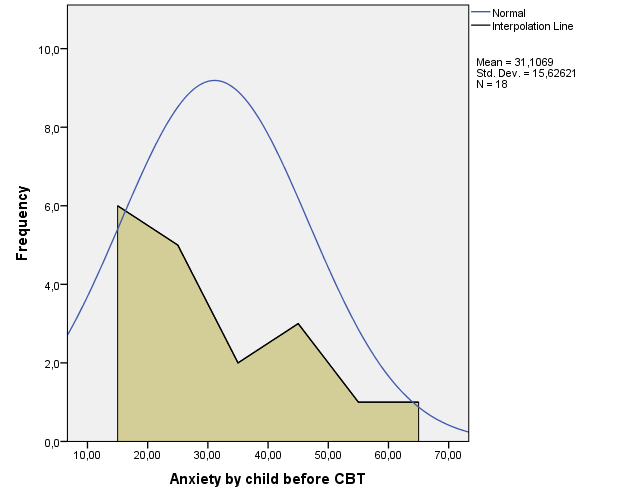
\includegraphics[width=0.8\textwidth]{STATS1B-HW4-Q5b-1}
            \caption{This (centred) histogram of the data from \texttt{anxc1} shows that it is a right-skewed distribution, with $\bar{x}=31.1069$, $s=15.62621$, and $n=18$.}
            \label{fig:hw4q5b}
        \end{figure}
        \FloatBarrier
    \end{enumerate}
\end{enumerate}

\subsection{Homework 5}
\begin{enumerate}
    \item Repeat the comparison of the QSHA scores of the first- and second-year psychology students in the homework Exercise 3 from last week, only this time use the pooled-variance $t$ test.
    \begin{enumerate}
        \item Perform the significance test and determine the $p$ value.
        \begin{framed}{\textbf{Solution}}
        Begin by computing the pooled variance:
        \begin{align}
            s_p^2 &= \frac{\brac{n_1 - 1}s^2_1 + \brac{n_2 - 1}s^2_2}{\brac{n_1 - 1} + \brac{n_2 - 1}} \\
            &= \frac{24 \times 4.89^2 + 28\times 5.65^2}{24 + 28} = \frac{1467.7204}{52} \approx 28.2254.
            \shortintertext{So our pooled standard deviation is $\sqrt{28.2254} \approx 5.313$ allowing us to compute the standard error:}
            se &= s_p \sqrt{\frac{1}{n_1} + \frac{1}{n_2}} = 5.313 \times \sqrt{\frac{1}{25} + \frac{1}{29}} \approx 1.45. \\
            \implies t &= \frac{131-127}{se} = \frac{4}{1.45} \approx 2.759 \sim t(52).
            \intertext{We can see from table $B$ that a $t$-statistic which is more extreme than 2.009 is significant at the 5\% level (noting that our null hypothesis is two-sided) for 50 degrees of freedom. In our case we have $n_1 + n_2- 2=52$ degrees of freedom, so it is not possible to directly read the critical $t$-value but we can assume that $2.759$ is a significant $t$-value. Using an online calculator, $t^*(52)=2.006647$ meaning that our $p$-value must be less than $0.05$ as it is less than our statistic. Indeed,}
            p &= \pr{\vbrac{t_{52}} > 1.952} = 0.007985.
        \end{align}
        \end{framed}
        
        \item Compute the 95\% confidence interval for the difference between the QHSA scores of first- and second-year psychology students.
        \begin{framed}{\textbf{Solution}}
        In the previous part, we calculated the critical $t$-value for 52 degrees of freedom as $2.006647$, so our 95\% CI for $\mu_d$ is
        \begin{align}
            \Bar{x}_1 - \bar{x}_2 \pm t^*_{52} \times se = 4 \pm 2.006647 \times 1.45 = 4\pm 2.91 = \brac{1.09 , 6.91}.
        \end{align}
        The probability that the true value of the parameter for the difference in means in the population lies between 1.09 and 6.91 is 0.950.
        \end{framed}
        
        \item Compare your results with the results in homework Exercise 3 of last week. How well do the results of the different two-sample $t$ procedures correspond?
        \begin{framed}{\textbf{Solution}}
        The samples are of similar (not equal) size, which accounts for how similar the Standard Errors are (1.434 for unpooled v.s. 1.45 for pooled). The main difference is the degrees of freedom used for the test: in the previous homework, we use 24 which resulted in a fatter tailed distribution, larger critical value and thus larger margin of error for the confidence interval. 
        \end{framed}
%%%%%%%%tikz here
    \end{enumerate}
    
    \item Due to a shooting incident in a Rotterdam supermarket where a member of the supermarket staff was shot, the supermarket wanted to determine whether the public thought supermarkets were safe. The following question was asked: ``Supermarkets should close at night for security reasons''. Of the 500 respondents, 156 answered with ``Yes'', and 344 with ``No''.
    \begin{enumerate}
        \item Compute the sample proportion that said ``Yes'', and estimate the standard deviation of that proportion.
        \begin{framed}{\textbf{Solution}}
        The sample proportion that said ``yes'' is the number of people who said ``yes'' divided by the total number of people in the sample:
        \begin{align}
            \Hat{\pi} &= \frac{156}{500} = 0.312.
            \intertext{The estimate for the standard deviation of the proportion (or standard error of the estimate) is given by the square root of the proportion that said ``yes'' times the proportion that said ``no'' divided by the sample size:}
            se &= \sqrt{\frac{\Hat{\pi} \brac{1-\Hat{\pi}}}{n}} = \sqrt{\frac{0.312 \times 0.688}{500}} = \sqrt{0.000429312} \approx 0.02072.
        \end{align}
        \end{framed}
        
        \item Use your answer to the previous question to find a 95\% confidence interval for the proportion people that advocate closing supermarkets at night.
        \begin{framed}{\textbf{Solution}}
        \begin{align}
            \text{95\% CI for $\pi$: } \Hat{\pi} \pm 1.96 \times se &= 0.312 \pm 1.96 \times 0.02072 \\
            &= \brac{0.2714 , 0.3526}.
        \end{align}
        The true proportion of the population that believe supermarkets should be closed at night for security reasons lies between 0.2714 and 0.3526 with probability of 0.95. As this does not constitute a majority vote, we decline to close supermarkets at night for security reasons. 
        \end{framed}
    \end{enumerate}
    
    \item A matched-pairs experiment is done that compared the taste of ``regular'' fresh coffee with the taste of Senseo coffee. Every participant tasted two unmarked cups of coffee, one of each kind of coffee. The tastings were done in a random order. Each participant was asked to tell which one of the two cups they preferred. Of the 60 participants, 26 preferred regular coffee, and 34 preferred the Senseo coffee. Assume that $p$ is the chance that a randomly taken person prefers ``regular'' fresh coffee over Senseo.
    \begin{enumerate}
        \item Test the claim that a majority of people prefer regular coffee. Note the $z$ statistic and the $p$-value.
        \begin{framed}{\textbf{Solution}}
        We will consider rejecting the assumption that there is no preference in favour of a majority of people preferring ``regular'' fresh coffee over Senseo if the $p$-value is less than our prescribed $\alpha$. We formulate our hypotheses:
        \[
        \begin{matrix}
        H_0 & : & p = 0.5 \\
        H_a & : & p>0.5.
        \end{matrix}
        \] 
        Next, we calculate the standard error of the estimate under the null hypothesis in a sample size of 60:
        \begin{align}
            se_0 &= \sqrt{\frac{p_0 \brac{1 - p_0}}{n}} = \sqrt{\frac{0.5^2}{60}} \approx 0.065.
            \intertext{Finally, we calculate our $z$-value:}
            z &= \frac{\Hat{p} - p_0}{se_0} = \frac{\sfrac{26}{60} - 0.5}{0.065} \approx -1.026.
            \intertext{Visualise this $z$-value on the standard normal distribution, and recall that \~68\% of the population data lies between $-1$ and 1. A two-sided $p$-value would be roughly $(100-68)\% = 32\%$, so the right-tailed $p$-value would be roughly $(50 + 68/2)\% = 84\%$ and the left-tailed would be roughly $(100-84)\%=16\%$. This allows us to already deduce that we will not be rejecting our null hypothesis. Keeping this in mind, we calculate the $p$-value as}
            p &= \pr{Z>-1.026}
            \shortintertext{As the standard normal distribution is symmetric about the mean of zero, we can solve this as}
            &= \pr{Z<1.026} = 0.847554,
        \end{align}
        which agrees with our theoretical calculation.
        \end{framed}
        
        \item Is this result significant, using $\alpha = 0.05$?
        \begin{framed}{\textbf{Solution}}
        $p>\alpha$, so yeah.
        \end{framed}
        
        \item Compute a 90\% confidence interval for p.
        \begin{framed}{\textbf{Solution}}
        \begin{align}
            \text{90\% CI for $p$: } \Hat{p} \pm 1.645 \times se &= \sfrac{26}{60} \pm 1.645 \sqrt{\frac{26 \times 34}{60^3}} \\
            &\approx 0.4\bar{3} \pm 1.645 \times 0.064 \\
            &= \brac{0.3281 , 0.5386}.
        \end{align}
        The true value of the chance that a randomly selected person from the population that prefers ``regular'' fresh coffee over Senseo lies between 0.3281 and 0.5386 with probability of 0.9. Note that $p_0 = 0.5$ is contained in the 90\% CI.  
        \end{framed}
        
        \item Using your two answers above, form your conclusion about whether a majority of people prefer fresh coffee.
        \begin{framed}{\textbf{Solution}}
        It appears that they do not care either way, as we do not reject the null hypothesis that the chance a randomly selected person prefers ``regular'' fresh coffee over Senseo is 50\%.
        \end{framed}
    \end{enumerate}
    
    \item Suppose that in a study on depression among children, the researchers wanted to show a relationship between the depression among children and the composition of the family. The researchers made a distinction between one- and two-parent families. The following table shows the results of the study. The variable $X$ refers to the number of children with a diagnosis of depression, and $n$ refers to the total number of families of that type.
    \FloatBarrier
    \begin{table}[h]
    \centering
    \begin{tabular}{l|c|c}
    Family type & $n$ & $X$ \\ \hline
    One-parent families & 74 & 6 \\
    Two-parent families & 226 & 13
    \end{tabular}
    \end{table}
    \FloatBarrier
    \begin{enumerate}
        \item For the one-parent families, compute the proportion of children suffering from depression.
        \begin{framed}{\textbf{Solution}}
        Let $\pi_1$ denote the proportion of children in one-parent families suffering from depression (note that this is conditional on the number of parents!!), so $\hat{\pi}_1 = \sfrac{6}{74}=0.\overline{081}\approx 0.0811$. That means that the sample proportion of children in one-parent families not suffering from depression is $(1-0.0811) = 0.\overline{918}\approx 0.9189$.
        \end{framed}
        
        \item For the two-parent families, compute the proportion of children suffering from depression.
        \begin{framed}{\textbf{Solution}}
        Let $\pi_2$ denote the proportion of children in two-parent families suffering from depression, so $\hat{\pi}_2 = \sfrac{13}{226}\approx 0.0575$. That means that the sample proportion of children in two-parent families not suffering from depression is $(1-0.0575)\approx 0.9425$.
        \end{framed}
        
        \item Compute a 95\%-confidence interval for the difference between these proportions.
        \begin{framed}{\textbf{Solution}}
        95\% CI for $\pi_1 - \pi_2$: 
        \begin{align}
            \Hat{\pi}_1 - \Hat{\pi}_2 \pm 1.96 \times \sqrt{\frac{\Hat{\pi}_1 \times \brac{1-\Hat{\pi}_1 }}{n_1} + \frac{\Hat{\pi}_2 \times \brac{1-\Hat{\pi}_2 }}{n_2}} &= 0.02356 \pm 1.96 \times \sqrt{0.001007 + 0.015488} \\
            &= 0.02356 \pm 1.96 \times 0.12843 \\
            &= \brac{-0.228 , 0.275}.
        \end{align}
        Note that we used unpooled standard error? This is because we do not assume homoskedasticity in the population as it is not plausible. 
        \end{framed}
        
        \item On the basis of your computations above, what are your conclusions regarding depression and family composition?
        \begin{framed}{\textbf{Solution}}
        The true value of the difference between the proportions lies near and about zero, and ranges from $-0.228$ to $0.275$ with probability 0.95. This allows us to conclude that there is no real difference in the chances a child will suffer from depression whether they have one- or two-parent families. You could loosely conclude that a child who has a one-parent family is not more likely to develop depression than a child who has two parents, and thus single parents do a ``good job'' at ensuring their childrens' happiness.
        \end{framed}
    \end{enumerate}
    
    \item Eisses and Kluiter's did a study on depression symptoms among nursing home residents [Eisses and Kluiter, 2002]. The researchers found that the percentage of elderly people undergoing treatment for depression is lower in Drenthe than in the rest of the Netherlands. It was suspected that the staff in Drenthe nursing homes needed better training to detect depression symptoms, so a study was conducted to evaluate the effect of training. Six nursing homes took part in the study. The staff from the nursing homes were assigned to either a control condition (no training) or an experimental condition (training to detect depression symptoms). Three nursing homes were assigned to the control condition, and three to the experimental condition.
    \\
    Before and after the training, the residents of the nursing home were interviewed by an independent clinical psychologist. Based on the reports of individual residents, the psychologist determined whether that resident was suffering from depression. Eisses and Kluiter used the independent psychologist's diagnoses to compare to the staff's diagnoses, but in this practicum we will only analyze the report of the independent psychologist.
    \\
    Open the file \texttt{5 - Depression Diagnosis.sav}.
    \FloatBarrier
    \begin{table}[h]
    \centering
    \begin{tabular}{l|l}
    \textbf{Variable} & \textbf{Description} \\
    \texttt{participant} & Participant number \\
    \texttt{exp} & 1=control group, 2=experimental group \\
    \texttt{depdiaB} & depression diagnosis before staff training: 1=yes, 2=no, 9=missing \\
    \texttt{depdiaA} & depression diagnosis after staff training: 1=yes, 2=no, 9=missing
    \end{tabular}
    \end{table}
    \FloatBarrier
    Some data is missing, due to the fact that the residents moved between interviews.
    \\
    One question of interest is: what proportion of residents of nursing homes in Drenthe suffer from depression?
    \begin{enumerate}
        \item To answer this question would you use the scores on the pre-training measure, the post-training measure, or both? Explain your answer.
        \begin{framed}{\textbf{Solution}}
        The scores on the pre-training measure would be most useful in answering this question, as we do not want that the additional staff training provides a confounding variable for us to solve. By doing so, we negate the allocation to control or experimental group and can simply estimate the proportion of residents of nursing homes in Drenthe suffering from depression. 
        \end{framed}
        
        \item Compute the proportion of residents suffering from depression before the training. Look closely at the frequency table. How many residents are diagnosed as depressed before the training? What percent is depressed?
        \begin{framed}{\textbf{Solution}}
        The first thing to notice is that 28 of 701 participants have missing data, so keeping that adjustment in mind the sample proportion is 0.045 even though there are 30 residents with depression in total. With respect to the total 4.3\% have depression, and when accounting for the missing data we have 4.5\%. The frequency table is given in \Cref{tab:hw5q5b}.
        \end{framed}
        \begin{figure}[h]
            \centering
            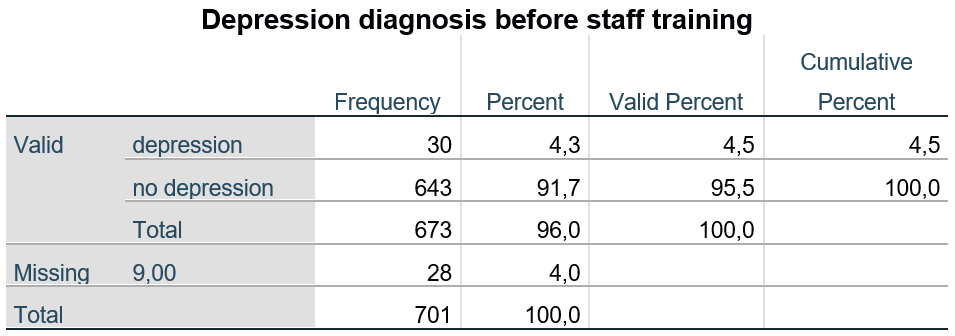
\includegraphics[width=0.68\linewidth]{STATS1BHW5Q5b-tabonly.png}
            \caption{SPSS frequency table output for the proportion of residents of nursing homes in Drenthe suffering from depression prior to initiating staff training in detecting symptoms of depression.}
            \label{tab:hw5q5b}
        \end{figure}
    \end{enumerate}
    These data will be used again in next week’s practicum.
\end{enumerate}

\subsection{Homework 6}
\begin{enumerate}
    \item Appleton, French and Vanderpump [Appleton et al., 1996] reported the results of a large epidemiological study of women in Great Britain. In the beginning of the 1970s, many women in Great Britain were asked about their health and health-related habits. Twenty years later, the women were contacted again to determine who had lived and who died. The table below shows the results.
    \FloatBarrier
    \begin{table}[h]
        \centering
        \begin{tabular}{c|cc}
             {} & Smoker & Non-smoker \\ \hline
             Dead & 139 & 230 \\
             Alive & 443 & 502 \\ \hline 
             Total & 582 & 732
        \end{tabular}
    \end{table}
    \FloatBarrier
    \begin{enumerate}
        \item Analyze the data, using plots and descriptive statistics. Use SPSS and/or R (hint: type in ``?prop.test'' in R and pay attention to the examples below) for your analysis. Describe what you did and sketch a copy of any informative plot you made.
        \begin{framed}{\textbf{Solution}}
        For obvious reasons, let's denote ``success'' as being alive, and failure as being ``dead'' with respect to table 8.6 from Agresti. So we have $\hat{\pi}_1 = 443/582 \approx 0.76117 $, $\hat{\pi}_2 = 502/732 \approx 0.68579 $, $\hat{\pi} = (443+502)/(582+732) = 945/1314 \approx 0.71918$ and $se_0 = \sqrt{\hat{\pi}\brac{1 - \hat{\pi}}\brac{\sfrac{1}{n_1} + \sfrac{1}{n_2}}} = \sqrt{0.71918\brac{1 - 0.71918}\brac{\sfrac{1}{582} + \sfrac{1}{732}}} \approx 0.02496$, which results in the $z$-statistic $\brac{\hat{\pi}_1 - \hat{\pi}_2}/se_0 = (0.76117 - 0.68579)/0.02496 \approx 3.02$. This $z$-statistic already indicates that $p<\alpha = 0.05$ and we will reject the null hypothesis ($H_0: \pi_1 = \pi_2$) and squaring gives $z^2=9.12$. 
        If you're using \texttt{R}, input the following code:\\
        \texttt{alive <- c(443,502)} \\
        \texttt{total <- c(582,732)} \\
        \texttt{prop.test(alive,total)} 
        \begin{center}
            \texttt{2-sample test for equality of proportions with continuity correction} 
        \end{center}
        \texttt{\quad data:  alive out of total \\
        \quad X-squared = 8.7515, df = 1, p-value = 0.003093 \\
        \quad alternative hypothesis: two.sided \\
        \quad 95 percent confidence interval: \\
        \quad  0.02555629 0.12519578 \\
        \quad sample estimates: \\
        \quad    prop 1    prop 2  \\
        \quad 0.7611684 0.6857923} \\
        You can use a bar graph of the sample percentages to display this information. 
        \end{framed}
        
        
        \item Based on the data in the table, what do you conclude?
        \begin{framed}{\textbf{Solution}}
        We assume that the population variables $\pi_1$ and $\pi_2$ are independent, i.e. smoking does not negatively influence the health of a woman (during that time period), and would expect that $\hat{\pi}_1 \approx \hat{\pi}_2$ in any sample from said population. 
        \end{framed}
        
    \FloatBarrier
    \begin{table}[h]
        \centering
        \begin{tabular}{c|cc}
             {} & Smoker & Non-smoker \\ \hline
             Dead & 23.88\% & 31.42\% \\
             Alive & 76.12\% & 68.58\% \\ \hline 
             Total & 100\% & 100\%
        \end{tabular}
    \end{table}
    \FloatBarrier
    \end{enumerate}
    
    \item In a longitudinal study of sexual orientation by [Golombok and Tasker, 1996], children of homosexual mothers were compared to children of heterosexual single mothers. The researchers asked the children about their sexual orientation when they were about 24 years old. The following table shows the children's sexual orientations as a function of the mothers' sexual orientations.
    \FloatBarrier
    \begin{table}[h]
        \centering
        \begin{tabular}{ll|cc}
            &  & \multicolumn{2}{c}{Mother} \\
            &  & Homosexual & Heterosexual \\ \hline 
            \multicolumn{1}{r}{\multirow{2}{*}{Child}} & Homosexual/bisexual & 2 (Expected: \underline{$1.1\bar{1}$}) & 0 (Expected: \underline{$0.8\bar{8}$}) \\
            \multicolumn{1}{r}{} & Heterosexual & 23 (Expected: \underline{$23.8\bar{8}$}) & 20 (Expected: \underline{$19.1\bar{1}$}) \\ \hline
            & Total & 25 & 20
        \end{tabular}
    \end{table}
    \FloatBarrier
    The SPSS file with these data is \texttt{6 - Golombok and Tasker.sav}.
    \begin{enumerate}
        \item Compute the expected frequencies under the assumption that the two factors are independent with SPSS. Note them in the previous table.
        \begin{framed}{\textbf{Solution}}
        You can calculate the expected frequencies using Bayes' Rule for Independence. First we denote $M_H$ as the event that the mother is homosexual and $M_S$ as the event that the mother is heterosexual. Similarly, $C_H$ denotes the event that the child is homo/bisexual and $C_S$ denotes the event that the child is heterosexual. The marginal probabilities can be found by adding the row or column frequencies and dividing by the sample size, e.g. $\pr{M_H} = 25/45$.
        \begin{align}
            \pr{A \cap B} &= \pr{A} \times \pr{B} .
            \intertext{The above formula is Bayes' Rule for Independence.}
            \implies \pr{M_H \cap C_H} &= \pr{M_H} \times \pr{C_H} = \frac{25}{45} \times \frac{2+0}{45} = \frac{50}{45^2} \approx 2.47\%. 
            \intertext{Assuming that the two factors are independent, we find that there is a 2.47\% chance that a homosexual mother will have a child that is homo/bisexual as well. We now know the probability of such an event, so multiplying it by the sample size will give the expected value. }
            \implies \E\brac{M_H \cap C_H} &= 45 \times 2.47\% = \frac{50}{45} = 1.1\bar{1}.
            \intertext{The expected number of homo/bisexual children who also have a homosexual mother is less than the observed value of 2, and is 1.11. The other probabilities are calculated in the following way:}
            \pr{M_S \cap C_H} &= \pr{M_S} \times \pr{C_H} = \frac{20}{45} \times \frac{2+0}{45} = \frac{40}{45^2} \approx 1.98\%. \\
            \pr{M_H \cap C_S} &= \pr{M_H} \times \pr{C_S} = \frac{25}{45} \times \frac{23+20}{45} = \frac{1075}{45^2} \approx 53.09\%. \\
            \pr{M_S \cap C_S} &= \pr{M_S} \times \pr{C_S} = \frac{20}{45} \times \frac{23+20}{45} = \frac{860}{45^2} \approx 42.47\%.
            \intertext{Which gives us the following expected values:}
            \implies \E\brac{M_S \cap C_H} &= 45 \times 1.98\% = \frac{40}{45} = 0.8\bar{8}. \\
            \E\brac{M_H \cap C_S} &= 45 \times 53.09\% = \frac{1075}{45} = 23.8\bar{8}. \\
            \E\brac{M_S \cap C_S} &= 45 \times 42.47\% = \frac{860}{45} = 19.1\bar{1}. 
        \end{align}
        \end{framed}
        
        \item Is a $\chi^2$ test appropriate for these data? Why or why not?
        \begin{framed}{\textbf{Solution}}
        No. We need the expected frequencies in each cell to be at least 5, or at least 10 for df=1.
        \end{framed}
        
        \item Use SPSS to perform the $\chi^2$ test and examine the output. Note it below. Notice that SPSS informs you about the number of cells with a frequency below five.
        \begin{framed}{\textbf{Solution}}
        
        \begin{align}
            \chi^2 &= \sum_{i=1}^k\frac{\brac{f_{0,i} - f_{e,i}}^2}{f_{e,i}}
            \shortintertext{$f_{0,i}$ denotes the \textit{observed} frequency and $f_{e,i}$ denotes the \textit{expected} frequency in cell $i$, where $i$ is the number of rows $r$ times the number of columns $c$ so here $i=2 \times 2=4$.}
            &=\frac{\brac{2 - 1.11}^2}{1.11} + \frac{\brac{0 - 0.89}^2}{0.89} + \frac{\brac{23 - 23.89}^2}{23.89} + \frac{\brac{20 - 19.11}^2}{19.11} \\
            &= \frac{0.89^2}{1.11} + \frac{0.89^2}{0.89} + \frac{0.89^2}{23.89} + \frac{0.89^2}{19.11}. \\
            &\approx 1.678. 
            \shortintertext{The $p$-value is calculated as follows:}
            p &= \pr{\chi^2_1 > 1.678} = 0.19519.
        \end{align}
        You can enter the following into R to achieve the same output: \\
        \texttt{x <- matrix(c(2,23,0,20), nrow=2) \\
         chisq.test(x,correct=FALSE)} 
         \begin{center}
             \texttt{Pearson's Chi-squared test}
         \end{center}
        \texttt{data:  x \\
        X-squared = 1.6744, df = 1, p-value = 0.1957} \\
        The use of \texttt{correct=FALSE} removes Yates' continuity correction. \\
        As $df = (r-1)\times (c-1) = 1$, we can also look at $z^2$: first calculate the standard error under the null hypothesis of $\pi_1 = \pi_2$:
        \begin{align}
            \hat{\pi} &= \frac{2}{45} \approx 0.0\bar{4}. \\
            \implies se_0^2 &= \hat{\pi}\brac{1-\hat{\pi}}\brac{\frac{1}{n_1} + \frac{1}{n_2}} \\
            &= 0.0\bar{4}\times 0.9\bar{5} \brac{\frac{1}{25} + \frac{1}{20}} = \frac{2 \times 43}{45^2} \times \frac{9}{100} = \frac{43}{11250} \approx 0.0038\bar{2}. \\
            \implies z^2 &= \frac{\brac{\hat{\pi}_1 - \hat{\pi}_2}^2}{se_0^2} \\
            &= \frac{\brac{\sfrac{2}{25} - \sfrac{0}{20}}^2}{0.0038222} = \frac{72}{43} \approx 1.6744.
            \intertext{We would have a significant result if the statistic $z^2$ is more extreme than $1.96^2 = 3.8416$ for $\alpha=0.05$, which it isn't. The $p$-value is calculated as follows:}
            p &= \pr{\chi^2_1 > 1.674} = 0.195724.
        \end{align}
        Neither $p$-value is significant at $\alpha = 0.05$ level - we do not reject the null hypothesis that they are independent
        \end{framed}
        
        \item The SPSS output also yields the result of Fisher's exact test. Note the result of this test, along with the relevant statistics.
        \begin{framed}{\textbf{Solution}}
        You can calculate this yourself using the hypergeometric distribution:
        \begin{align}
             p_1 &= \frac{2! 43! 25! 20!}{2!0!23!20!45!} \approx 0.303030
            \intertext{As 2 is the greatest possible number for this cell, keeping the marginal frequencies the same (other possibilities are 1 and 0), this is the right-tailed $p$-value. Next, you need to calculate the $p$-values for different extremes \textit{without altering the marginal frequencies}, i.e. altering only the cell frequencies:}
            p_2 &= \frac{2! 43! 25! 20!}{1!1!24!19!45!} \approx 0.50505.  \\
            p_3 &= \frac{2! 43! 25! 20!}{0!2!25!18!45!} \approx 0.191919.
            \intertext{If you added all the $p$-values together, you would get the left-tailed $p$-value\footnotemark. If you add together the $p$-values of all combinations that have lower probabilities than that of the observed data (so $p$-values less than $0.303030 = p_1$), you get the two-tailed $p$-value. The only $p$-value that is smaller than $p_1$ is $p_3$ (so for $\cbrac{(0,2), (25,18)}$), hence we add $p_1$ and $p_3$ together to get the two-tailed $p$-value:}
            p &= 0.30303 + 0.191919 = 0.494949.
        \end{align}
        You can do this in R: \\
        \texttt{x <- matrix(c(2,23,0,20), nrow=2) \\
         exact2x2(x,tsmethod="minlike")}
         \begin{center}
             \texttt{Two-sided Fisher's Exact Test (usual method using minimum likelihood)}
         \end{center}
         \texttt{data:  x\\
         p-value = 0.4949\\
         alternative hypothesis: true odds ratio is not equal to 1\\
         95 percent confidence interval:\\
         0.2316 \quad Inf\\
         sample estimates:\\
         odds ratio \\
        ${}$ \quad Inf} \\
        Note that the confidence interval given is unbounded as it tends to $\infty$? This is because of the inclusion of the zero in our table: the odds ratio is $OR = (2/23)/(0/20) = (2/23) \times (20/0) = \infty$ and everyone knows you can't divide by zero. The computation of the 95\% Confidence Interval for the odds ratio is as follows:
        \begin{align}
            se_{\ln{\brac{OR}}} &= \sqrt{\frac{1}{2} + \frac{1}{0} + \frac{1}{23} + \frac{1}{20}} = \sqrt{\infty}. 
            \shortintertext{95\% CI for odds ratio:}
            \exp{\cbrac{\ln{\brac{OR}} \pm 1.96 \times se_{\ln{\brac{OR}}}}} &= \exp{\cbrac{\ln{\brac{\infty}} \pm 1.96 \times \sqrt{\infty}}} \\
            &= \brac{\infty \times e^{-1.96 \times \sqrt{\infty}} , \infty \times e^{1.96 \times \sqrt{\infty}}} \\
            &= \brac{0.2316 , \infty}.
        \end{align}
        This issue is not present when you don't have zero values in the table - a rearrangement of the columns does not aid us any further as we still have the zero in the odds ratio and the computation of the standard error. 
        \end{framed}
        \footnotetext{You can play around with the following applet to see what I mean with left- and right-tailed $p$-values: \url{https://istats.shinyapps.io/FisherExact/}.}
        
        \item Fisher's exact test was developed by the famous statistician R.A. Fisher. It is designed to test the same null hypothesis as the $\chi^2$ test, but it does not have the same problems with low cell counts that the $\chi^2$ test has. In this class you will not learn the details of how to compute the test by hand, but notice that SPSS gives a $p$ value for the test every time you compute a $\chi^2$ test. What do you conclude on the basis of Fisher's exact test?
        \begin{framed}{\textbf{Solution}}
        Fisher's exact test starts by computing the probabilities of \textit{all possible outcomes which do not alter the marginal frequencies} ($p_1$, $p_2$ and $p_3$), and adding all of these equates to the probability of all events, thus equals 1. For this reason, it is called \textit{exact} as you can exactly calculate the probability of any event using the actual (hypergeometric) sampling distribution rather than a normal approximation. The sampling distribution is not symmetric for low $n$, meaning that left-, right-, and two-tailed $p$-values do not add up to 1.
        \end{framed}
        
        \item It is also true that confidence intervals computed using small sample sizes can be quite inaccurate. What implications does this have for designing studies using two-way data?
        \begin{framed}{\textbf{Solution}}
        They are inaccurate due the lack of central tendency and presence of skew, also having a zero in the computation of the odds ratio (and therefore confidence interval) is really hard to work with, as written above. 
        \end{framed}
    \end{enumerate}
\end{enumerate}